A qualitative error analysis was conducted on the predictions made by both the XGBoost 2 and SVM 1 models to gain insight into their capabilities and weaknesses when applied to the SEM 2012 circle test set. Performing such an analysis is crucial when building a negation classifier due to the complex semantic nature of negation, which interacts with various aspects of meaning and sentence structure \cite{hossain2020predicting, cruz2016machine}.
\begin{figure}[!h]
\centering
    \makebox[\textwidth][c]{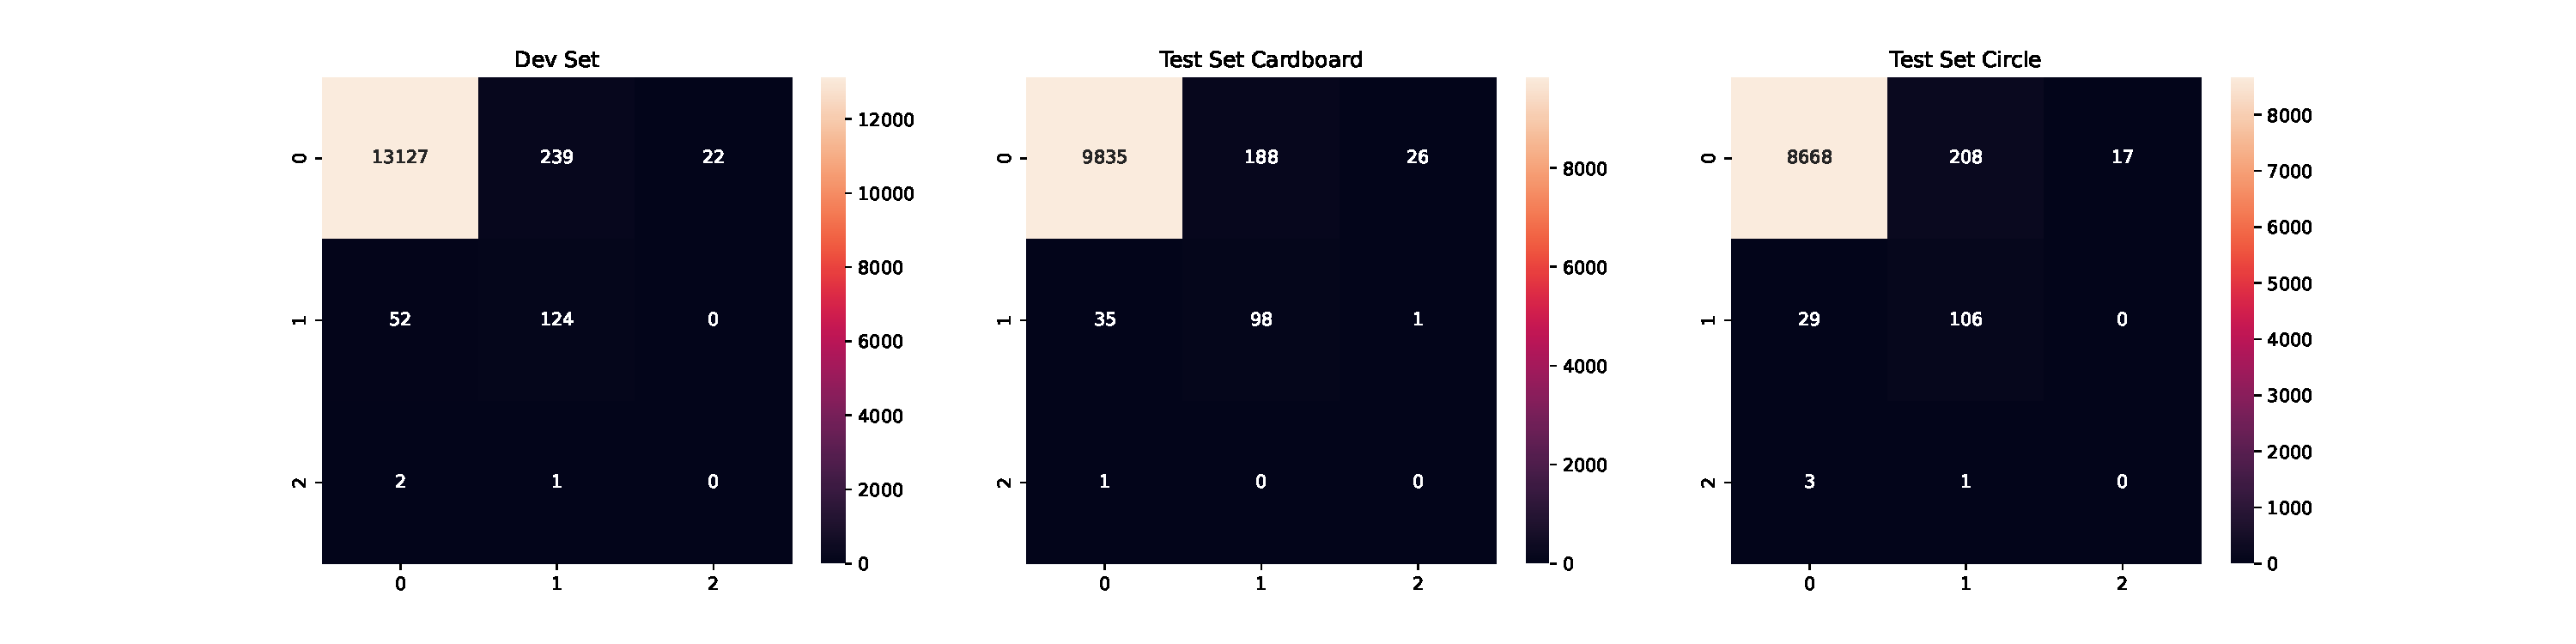
\includegraphics[width=1.3\textwidth]{Plots and results/Confusion_Matrix_svm.pdf}}
  \caption{Confusion Matrices Best Selected SVM}
  \label{fig:best_svm}
\end{figure}


\begin{table}[!h]
\caption{\label{tab:fns}Sample of false negatives in test set predictions}
\centering
\begin{tabular}{ccccc}
\hline
                                        Sentence &    Token & Golden Label & \begin{tabular}[c]{@{}l@{}}Prediction\\ (SVM)\end{tabular} & \begin{tabular}[c]{@{}l@{}}Prediction\\ (XGBoost)\end{tabular} \\
\hline
                  `` I do n't understand that . &      n't &  B-NEG &              O &              O \\
       You do n't object to tobacco , I take it ? &      n't &  B-NEG &              O &              O \\
                      I ca n't sleep for fright . &      n't &  B-NEG &              O &              O \\
                     `` I 'll have no more of it ! &     more &  I-NEG &              O &              O \\
                    That ca n't be all , Watson ? &      n't &  B-NEG &              O &              O \\
 ` If not , I 'll have no more to do with you . ' &     more &  I-NEG &              O &              O \\
         At first I thought that it was dislike . &  dislike &  B-NEG &              O &              O \\
\hline
\end{tabular}
\end{table}
Examining the false positive (FP) and false negative (FN) errors is particularly informative. An FP error occurs when the classifier identifies a negative cue token that is not annotated as such in the dataset, while an FN error takes place when the system fails to identify a token annotated as a negative cue.

\begin{table}[!h]
    \centering
    \caption{\label{tab:fps}Sample of false positives in test set predictions}
\begin{tabular}{ccccc}
\hline
                                          Sentence &      Token & Golden Label & \begin{tabular}[c]{@{}l@{}}Prediction\\ (SVM 1)\end{tabular} & \begin{tabular}[c]{@{}l@{}}Prediction\\ (XGBoost 2)\end{tabular} \\
\hline
           It sounds plausible , does it not ? &        not &      O &          B-NEG &          B-NEG \\
       Yes , here we are -- three days later . &       days &      O &          B-NEG &          B-NEG \\
      `` No doubt , sir ; but this is different . &         No &      O &          B-NEG &          B-NEG \\
      `` No doubt , sir ; but this is different . &          . &      O &          B-NEG &          B-NEG \\
         Then comes something much more definite : &  something &      O &          B-NEG &          B-NEG \\
  `` That was bad enough , but worse was to come . &       come &      O &          I-NEG &          I-NEG \\
                       One A , two B , and so on . &        and &      O &          B-NEG &          B-NEG \\
                    One A , two B , and so on . &         so &      O &          B-NEG &          B-NEG \\
                             You will hear soon . &        You &      O &          B-NEG &          B-NEG \\
                             You will hear soon . &       hear &      O &          B-NEG &          B-NEG \\
                                Is it not so ? '' &         '' &      O &          B-NEG &          B-NEG \\
              Your presence here was desirable . &          . &      O &          B-NEG &          B-NEG \\
 It was fear -- a deep , secret , shrinking fear . &     secret &      O &          B-NEG &          B-NEG \\

\hline
\end{tabular}
\end{table}
For XGBoost, the FP errors include 341 instances of B-NEG and 16 instances of I-NEG when the golden label is O. In comparison, SVM has 208 FP errors for B-NEG and 17 for I-NEG with the golden label as O. On the other hand, FN errors for XGBoost consist of 38 instances where the prediction is O, and the golden label is B-NEG, and 3 instances where the golden label is I-NEG. SVM presents a similar distribution with 29 FN errors for B-NEG and 3 for I-NEG when the model prediction is O, as seen in figures \ref{fig:best_svm} and \ref{fig:best_xgb}.

The errors observed in the test set predictions, as illustrated in tables \ref{tab:fns} and \ref{tab:fps}, could be attributed to both the complexity of negation, such as token \textit{n't}, which Cruz et al. (2016) \cite{cruz2016machine} defines as incorrect classification of a \textit{multiword cue}, and the distribution of the target variable. The current research utilized SVM and XGBoost models that incorporated semantic and syntactic features to account for this complexity, but some errors remained. Additionally, despite implementing methods to counteract the class imbalance issue in the training data, there were still insufficient examples for the algorithms to effectively learn from, which may have contributed to these persisting misclassifications.

To address these errors and improve the classifier's performance, additional data could be added to both the training set and test set to balance the distribution of the target variable. This would help reduce the problem of class imbalance in the dataset, leading to better model generalization.

\begin{figure}[!h]
\centering
    \makebox[\textwidth][c]{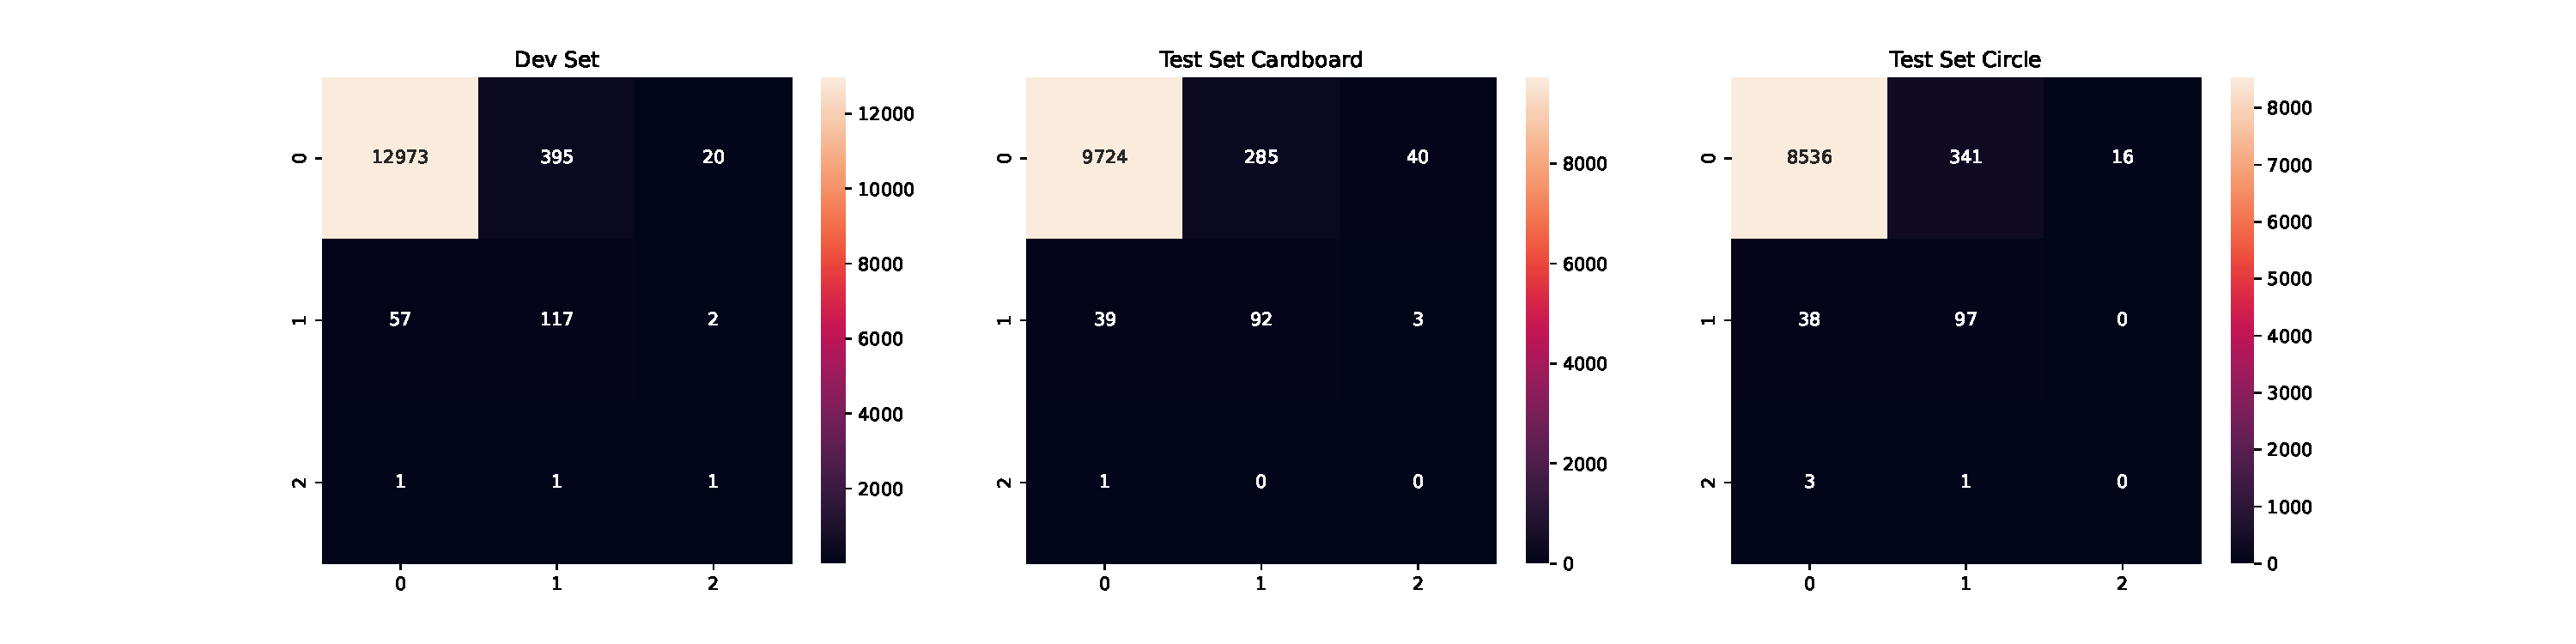
\includegraphics[width=1.3\textwidth]{Plots and results/Confusion_Matrix_xgb.pdf}}
  \caption{Confusion Matrices Best Selected XGBoost}
  \label{fig:best_xgb}
\end{figure}

